
==============================================

%TODO Apresentar o grafo de Clebsch H = (V_h,E_h), e o supergrafo de Clebsch H^* = (V,E^*)
%Apresento o artigo 
% Escolher um conjunto de vértices ruins e mostrar que sem ele o grafo possui homomorfismo ao C_5 (não confundir com humormofismo)
% 
%TODO mostrar a definição básica de [16]
%TODO precisa dizer que estamos buscando um homomorfimo no grafo de Clebsch H, e portanto, uma configuração é uma sequência de vértices de H.
% A \emph{configuration} $c$ is a sequence \(c_1,\ldots,c_n\) of positive integers in \([16]\).
A \emph{configuration} $c$ is a sequence \(c_1,\ldots,c_n\) of vertices of \(H\).
%colors of size $n$ where $c_i$ is the i-th element of the sequence and $c_i \in [1...16] | \forall i \in \{1..n\}$.

Given a rooted tree $T$ in $r$ of height $h$ where $r$ has three children and every other vertex has two children we can see that any connected subgraph of a graph G 


Given a 3-regular graph $G=(V,E)$ of girth at least $\girth$, we can see that any subgraph defines a rooted tree $T=(V',E')$ of height $h \leq gir$ where the root $r$ has tree children and every other vertex has two.
We can define the maximal tree $T_{max}$ has the tree with $h=gir$.
Henceforward, we shall call the rooted trees of this characteristics as simply trees.






=====================================

%%% Supergrafo, não agora 
%Let \(V_i = \{u\in V(H_0) : f_0(u) = i\}\)  for \(i\in V(C_5)\),
%and let \(H_0^+\) be the graph obtained from \(H_0\) by adding all the missing edges between the sets \(V_i\) and %\(V_j\) with \(ij \in E(C_5)\). 
%Let \(E^+\) be the set of these missing edges,
%and let \(H^+ = H\cup E^+\), and note that \(H\subseteq H^+\) and \(H\neq H^+\),
%while \(H^+ \setminus B_0 = H_0^+\) and \(f_0\) is a homomorphism of \(H_0^+\) to \(C_5\).
%In this work we approach the pentagon problem proving that every cubic graph with girth at least 17 has an homomorphism %to \(H_0^+ - 0\).
%In particular, the vertex \(0\) plays an important role throughout this work.


%( Mostrar no pyhton o homomorfismo)
% Definitrions





%TODO Definir N_r(u) e N_r[u]
%Let \(G\) be a cubic graph of girth \(\girth\).
%Given \(u\in V(G)\) and a positive integer \(r < g/2\),
%let \(T_u\) the subgraph of \(G\) consisting of all the vertices with distance at most \(r\) from \(u\),
%i.e., let \(N_r[u] = \{v \in V(G) : \dist(u,v) \leq r\}\),
%and put \(T_u = G[N_r[u]]\).
%Since \(G\) has girth \(\girth\), \(T_u\) is a tree.

% Motivação do algoritmo
%Let \(c\colon V(G)\to V(H)\).
%We define the \emph{cost} \(f(x)\) of a vertex \(x\in V(G)\) in \(c\)
%as \(1\) if \(c(x)\in\bads\) and \(0\) otherwise.
%Futhermore, we define the cost of \(c\) as the sum \(f(c) =\sum_{x\in V(G)}f(x)\).
%Now, let \(c\colon V(G) \to V(H)\) be a homomorphism that minimizes \(f(c)\),
%and suppose that there is a coloring \(c'\colon V(T_u) \to V(H)\) such that the following holds
%\begin{enumerate}
%    \item \(\{c'(x),c'(y)\}\in E(H)\) for every \(xy\in E(T_u)\);
%    \item \(c'(x) = c(x)\) for all \(x\in N_r(u)\). 
%\end{enumerate}
%The \emph{\(r\)-local cost} of a map \(m\colon V(T_u) \to V(H)\) is the value \(f'(m) = \sum_{x\in V(T_u)} f(x)\).
%Consider the map \(c^*\)
%defined by \(c^*(x) = c'(x)\) if \(x\in V(T_u)\)
%and \(c^*(x) = c(x)\) otherwise.
%If \(f'(c') < f'(c)\), then \(c^*\)
%is a homomorphism of \(G\) in \(H\) such that \(f(c^*) = f(c) - f'(c) + f'(c') < f(c)\),
%a contradiction to the minimality of \(c\).
%
%
%================================




==============================================


The coloring $cor$ of one of such trees is defined has the mapping $cor: V' \rightarrow V(Clebsch graph)$ such that for every pair $(x,y) \in E'$ we have that $ (cor(x), cor(y)) \in E(Clebsch graph)$. Given an Tree $T_u$, we denote by $level_i$ the sequence of all vertices of \(T\) that are at distance precisely $i$ of the root. With a coloring $cor_x$ the sequence of vertices $x \in level_i$ defines a configuration $cor_x(v) \forall v \in level_i$.

A configuration ascending and descending 


We can define a viable configuration $c$ as one such that we can construct a tree that, for some $level_i$ and some coloring $cor_x$, we can contruct the configuration. For any viable configuration, we can define the family of related colorings such that for any given tree the $cor(T)$ at $level_i$ is $c$.


-->An example of an unviable and a viable configuration with tree vertices 



Given a set $\mathfrak{B}$ of bad vertices, we define the a indicator function over the set $\{1...16\}$ cost as:
\[ 
cost(v) = 
     \begin{cases}
       1 &\quad\text{if } v\in \mathfrak{B}\\
       0 &\quad\text{if } v\notin \mathfrak{B}\\
     \end{cases}\]

And function of cost given a tree such as:  
\[ Cost(T) = \sum_{v \in V'}cost(cor(v)) \]



\subsection{Definition of Substitution}
Given a configuration $c$, we can define $Subst(c,index,x)$  as the the operation that defines a new configuration $cn$ where $cn_i = c_i if i \neq index else x$.   

\subsection{Definition of Sub-problem}
Given a set $\mathfrak{C}$ of configurations on level n, we can divide the subset between $\mathfrak{C_g}$ = $\{ c | c \in \mathfrak{C},  RC(c)  < FC(c) \}$ and  $\mathfrak{C_b}=\{ c | c \in \mathfrak{C},  FC(c) \geq RC(c) \}$. We can define a good substitution pair $(index, x)$ one as such that $c \in \mathfrak{C_b}$ and $Subst(c,index,x) \in \mathfrak{C_g}$. Given a configuration $c$ we have the set of good substitutions pairs as $ \{ (index, x) | index \in [1...n],  x \in c, Subst(c,index,x) \in \mathfrak{C_g} \}$. We can summarize the sub-problem as, given a configuration $c \in \mathfrak{C_b}$ and a color $y \in c$, if any descendent configuration $c_m$ on level $n+m$ has a ascendant $c_a$ configuration such that $c_a \in Subst(c,index(y),x)$.

\subsection{Using Substitution to solve}


a local operation that excludes certain vertices from a homomorphism that takes a subcubic graph of girth at least $g$ to an graph $G$. And if that operation is always possible to subcubic graph of girth at least $g$, than we are able to conclude that there is always a homomorphism from any such graph to $G$ without the excluded vertices. 

In order to build upon the results of Theorem \ref{thm:DevosSamal11}, we define the \emph{Enhanced Clebsch Graph} $H^{+}$ as the graph formed by adding the following set of edges \[\{(3, 15),(4, 9),(6, 9),(6, 10),(6, 13),(8, 10),(9, 15),(10, 15)\}\] to the Clebsch Graph as show in Figure \ref{fig:enhanced_clebsch_graph}. 
It' clear from the definition that every edge in $H$ also exists in $H^{+}$, as a natural consequence, Theorem \ref{thm:DevosSamal11} can be generalized do $H^+$. 

\begin{figure}
    \centering
    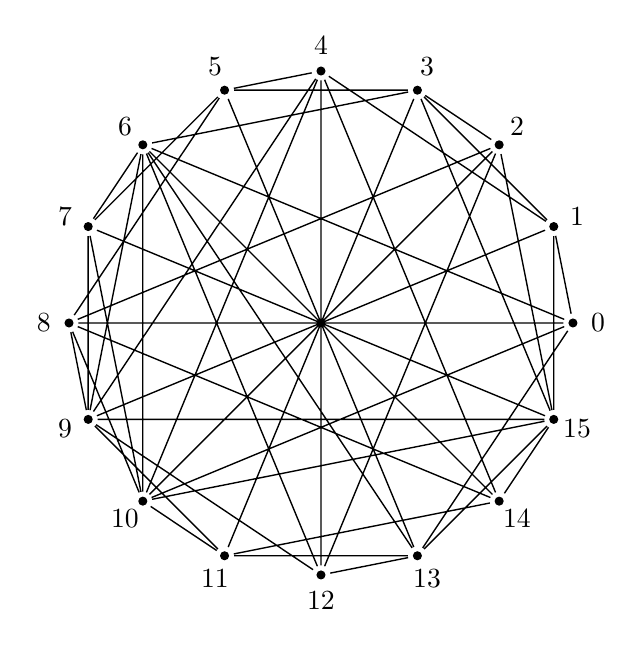
\begin{tikzpicture}[node distance=2cm,scale = .8]
% Vértices
\tikzset{black vertex/.style={circle,draw,minimum size=1mm,inner sep=0pt,outer sep=2pt,fill=black, color=black}}

\foreach \x in {0,...,15}{
    \node[black vertex] (\x) at (\x*360/16:4) {};
	\node () at (\x*360/16:4.4) {\x};
}


% \draw[line width = .5pt] (0) -- (1) (2) -- (3) (4) -- (5) (6) -- (7) (8) -- (9) (10) -- (11) (12) -- (13) (14) -- (15);

\draw[line width = .5pt] (0) -- (1) (0) -- (6) (0) -- (8) (0) -- (10) (0) -- (13) (1) -- (3) (1) -- (4) (1) -- (9) (1) -- (15) (2) -- (3) (2) -- (8) (2) -- (10) (2) -- (12) (2) -- (15) (3) -- (5) (3) -- (6) (3) -- (11) (4) -- (5) (4) -- (10) (4) -- (12) (4) -- (14) (5) -- (7) (5) -- (8) (5) -- (13) (6) -- (7) (6) -- (12) (6) -- (14) (7) -- (9) (7) -- (10) (7) -- (15) (8) -- (9) (8) -- (14) (9) -- (11) (9) -- (12) (10) -- (11) (11) -- (13) (11) -- (14) (12) -- (13) (13) -- (15) (14) -- (15)
(3) -- (15) (4) -- (9) (6) -- (9) (6) -- (10) (6) -- (13) (8) -- (10) (9) -- (15) (10) -- (15);


\end{tikzpicture}
    \caption{Enhanced Clebsch graph}
    \label{fig:enhanced_clebsch_graph}
\end{figure}

In what follows, we denote by \(B_0\) the set of vertices $\{0,1,2,7,12\}$,
and by \(H_0\) the graph obtained from \(H^{+}\) by removing the vertices in \(B_0\).
It's not hard to check that \(H_0\) has a homomorphism \(h_0\) to $C_5$,
and hence, to solve \nesetril{} Pentagon Problem, it's enough to prove that there is a constant \(g_0\) such that every cubic graph with girth at least \(g_0\) has an homomorphism to \(H_0\),
i.e., an homomorphism to \(H\) that avoids the vertices in \(B_0\).


The motivation of this work is to show that every cubic graph of girth at least \(17\) has an homomorphism to the Enhanced Clebsch Graph that avoids a subset $\bads \subseteq B_0$, which improves the result of \cite{devos2011high} towards the Pentagon Problem. In the following, we proof the Theorem~\ref{thm:main} for $\bads=\{0\}$. 